%%%%%%%%%%%%%%%%%%%%%%%%%%%%%%%%%%%%%%%%%%%%%%%%
% %
% % Welcome to Overleaf --- just edit your LaTeX on the left,
% % and we'll compile it for you on the right. If you open the
% % 'Share' menu, you can invite other users to edit at the same
% % time. See www.overleaf.com/learn for more info. Enjoy!
% %
% % Note: you can export the pdf to see the result at full
% % resolution.
% %
% %%%%%%%%%%%%%%%%%%%%%%%%%%%%%%%%%%%%%%%%%%%%%%%%%%%%%%%%%%%%%%%
% % Red-black tree
% % Author: Madit
% \documentclass{article}
% \usepackage{tikz}
% %%%<
% \usepackage{verbatim}
% \usepackage[active,tightpage]{preview}
% \PreviewEnvironment{tikzpicture}
% \setlength{\PreviewBorder}{10pt}%
% %%%>
% \begin{comment}
% :Title: Red-black tree
% :Tags: Trees;Graphs
% :Author: Madit
% :Slug: red-black-tree

% A red-black tree is a special type of binary tree, used in computer science
% to organize pieces of comparable data, such as text fragments or numbers.
% (Wikipedia)
% \end{comment}
% \usetikzlibrary{arrows}

% \tikzset{
%   treenode/.style = {align=center, inner sep=0pt, text centered,
%     font=\sffamily},
%   arn_n/.style = {treenode, circle, white, font=\sffamily\bfseries, draw=black,
%     fill=black, text width=1.5em},% arbre rouge noir, noeud noir
%   arn_r/.style = {treenode, circle, red, draw=red, 
%     text width=1.5em, very thick},% arbre rouge noir, noeud rouge
%   arn_x/.style = {treenode, rectangle, draw=black,
%     minimum width=0.5em, minimum height=0.5em}% arbre rouge noir, nil
% }

% \begin{document}
% \begin{tikzpicture}[->,>=stealth',level/.style={sibling distance = 5cm/#1,
%   level distance = 1.5cm}] 
% \node [arn_n] {33}
%     child{ node [arn_r] {15} 
%             child{ node [arn_n] {10} 
%             	child{ node [arn_r] {5} edge from parent node[above left]
%                          {$x$}} %for a named pointer
% 							child{ node [arn_x] {}}
%             }
%             child{ node [arn_n] {20}
% 							child{ node [arn_r] {18}}
% 							child{ node [arn_x] {}}
%             }                            
%     }
%     child{ node [arn_r] {47}
%             child{ node [arn_n] {38} 
% 							child{ node [arn_r] {36}}
% 							child{ node [arn_r] {39}}
%             }
%             child{ node [arn_n] {51}
% 							child{ node [arn_r] {49}}
% 							child{ node [arn_x] {}}
%             }
% 		}
% ; 
% \end{tikzpicture}
% % \begin{tikzpicture}
% %     \node[]{A} 
% %     child{ node [] {47}
% %         child{ node [] {38} 
% %                     child{ node [] {36}}
% %                     child{ node [] {39}}
% %     }
% %         child{ node [] {51}
% %                     child{ node [] {49}}
% %                     child{ node [] {}}
% %     }
% % };
% % \end{tikzpicture}
% \begin{tikzpicture}
%     [level/.style={sibling distance = 5cm/#1,level distance = 1.5cm}]
%     \node[]{A}
%     child{node[] {B}
%         child{node[]{D}}
%         child{node[]{E}
%             child{node[]{F}}
%             child[missing]
%         }
%     }
%     child{node[]{C}
%         child{node[]{G}}
%         child{node[]{H}
%             child{node[]{J}
%                 child{node[]{L}}
%                 child[missing]
%             }
%             child{node[]{K}}
%         }
%     };
% \end{tikzpictur

\documentclass{article}
\usepackage{tikz}
\usepackage{fullpage}
% \usepackage[active,tightpage]{preview}
% \PreviewEnvironment{tikzpicture}
% \setlength{\PreviewBorder}{10pt}
\usetikzlibrary{arrows,decorations.pathmorphing,backgrounds,positioning,fit,petri}


\begin{document}

% \usegdlibrary {trees}
\begin{tikzpicture}
    \node[circle,draw] (a) {};
    \node[circle,draw] (c)[above right =of a] {};
    \node[circle,draw] (b)[below right =of c] {};
    \node[circle,draw] (d)[below left =of a] {};
    \node[circle,draw] (e)[below right =of b] {};
    \path[-] (a) edge node{} (b)
                edge node{} (d)
                edge node{} (c)
            (b) edge node{} (c)
                edge node{}(e);
\end{tikzpicture}
\begin{tikzpicture}
    \node[circle,draw] (a) {};
    \node[circle,draw] (c)[above  =of a] {};
    \node[circle,draw,node distance=.25cm] (b)[right =of a] {};
    \node[circle,draw] (d)[below  =of a] {};
    \node[circle,draw] (e)[right =of d] {};
    \path[-](a) edge node{}(c)
                edge node{}(b)
                edge node{}(d)
            (b) edge[in=30, out=30] node{}(c)
                edge node{}(e);
\end{tikzpicture}
\begin{tikzpicture}
    \node[circle,draw] (a){};
    \node[circle,draw] (b)[above =of a]{};
    \node[circle,draw] (c)[below =of a]{};
    \node[circle,draw] (d)[above right =of a]{};
    \node[circle,draw] (e)[below right =of a]{};
    \path[-] (a) edge node{}(b)
                edge node{}(c)
                edge node{}(d)
                edge node{}(e);
\end{tikzpicture}
\begin{tikzpicture}
    \node[circle,draw] (a){};
    \node[circle,draw] (b)[above right =of a]{};
    \node[circle,draw] (c)[below right =of a]{};
    \node[circle,draw] (d)[above left =of a]{};
    \node[circle,draw] (e)[below left =of a]{};
    \path[-] (a) edge node{}(b)
                edge node{}(c)
                edge node{}(d)
                edge node{}(e);
\end{tikzpicture}
\begin{tikzpicture}
    \node[circle,draw] (a) {};
    \node[circle,draw] (c)[above right =of a] {};
    \node[circle,draw] (b)[below right =of c] {};
    \node[circle,draw] (d)[below left =of a] {};
    \node[circle,draw] (e)[below right =of b] {};
    \path[-] (a) edge node{} (b)
                edge node{} (d)
                edge node{} (c)
            (b) edge node{} (c)
                edge node{}(e);
    \node[node distance=.75cm](anchor)[right =of b]{};
    \node[circle,draw] (i)[right =of anchor] {};
    \node[circle,draw] (j)[above  =of i] {};
    \node[circle,draw,node distance=.25cm] (k)[right =of i] {};
    \node[circle,draw] (l)[below  =of i] {};
    \node[circle,draw] (m)[below right =of i] {};
    \path[-](i) edge node{}(j)
                edge node{}(k)
                edge node{}(l)
            (k) edge[in=30, out=30] node{}(j)
                edge node{}(m);

\end{tikzpicture}
\begin{tikzpicture}
    \node[circle,draw] (a){};
    \node[circle,draw] (b)[above =of a]{};
    \node[circle,draw] (c)[below =of a]{};
    \node[circle,draw] (d)[above right =of a]{};
    \node[circle,draw] (e)[below right =of a]{};
    \path[-] (a) edge node{}(b)
                edge node{}(c)
                edge node{}(d)
                edge node{}(e);
    \node[node distance=1.5cm](anchor)[right =of a]{};
    \node[circle,draw] (aa)[right =of anchor]{};
    \node[circle,draw] (bb)[above right =of aa]{};
    \node[circle,draw] (cc)[below right =of aa]{};
    \node[circle,draw] (dd)[above left =of aa]{};
    \node[circle,draw] (ee)[below left =of aa]{};
    \path[-] (aa) edge node{}(bb)
                edge node{}(cc)
                edge node{}(dd)
                edge node{}(ee);
\end{tikzpicture}
\begin{tikzpicture}[>=stealth]
    \node(a) {};
    \node(b)[below =of a] {};
    \node(c)[right =of a] {};
    \path[->] (b) edge node{}(a)
    (a)edge node {}(c);
\end{tikzpicture}
\begin{tikzpicture}
    \node[circle,draw](a){A};
    \node[circle,draw](c)[above right =of a]{C};
    \node[circle,draw](b)[below right =of c]{B};
    \node[circle,draw](d)[below right =of a]{D};
    \path[-](a) edge node{}(c)
                edge [bend right] node {}(c)
                edge node{}(b)
                edge node{}(d)
                edge[bend left] node {}(d)
            (b)edge node{}(c)
            edge node{}(d);
    \draw[dashed] (-1,1)--(4,1);
    \draw[dashed] (-1,-1)--(4,-1);
\end{tikzpicture}
\begin{tikzpicture}
    \node[circle,draw](a){a};
    \node[circle,draw, node distance = 3cm](b)[right =of a]{b};
    \node[circle,draw, node distance =.5cm](c)[below right =of a]{c};
    \node[circle,draw, node distance = 2cm](d)[below =of a]{d};
    \node[circle,draw, node distance = 3cm](e)[right =of d]{e};
    \node[circle,draw, node distance =.5cm](f)[above left =of e]{f};
    \path[-](b) edge node{}(a)
                edge node{}(e)
                edge node{}(c)
                edge node{}(f)
            (d)edge node{}(a)
                edge node{}(e)
                edge node{}(c)
                edge node{}(f);
    \node(anchor)[right=of b]{};
    \node[circle,draw](aa)[right =of anchor]{aa};
    \node[circle,draw](bb)[right =of aa]{b};
    \node[circle,draw](cc)[right =of bb]{c};
    \node[circle,draw](dd)[below =of aa]{d};
    \node[circle,draw](ee)[right =of dd]{e};
    \node[circle,draw](ff)[right =of ee]{f};
    \path[-](bb)edge node{}(aa)
                edge node{}(cc)
                edge node{}(dd)
                edge node{}(ff)
                edge node{}(ee)
            (dd)edge node{}(aa)
                edge node{}(ee)
            (ff)edge node{}(cc)
                edge node{}(ee);
\end{tikzpicture}
\begin{tikzpicture}
    [place/.style={circle,draw,fill=black!50}]
    \node[place] (a){};
    \node[node distance=.25cm] (text1)[below =of a]{$ k_1 $};
    \node[place] (b)[right=of a]{};
    \node[place] (c)[right=of b]{};
    \node[node distance=.25cm] (text2)[below right =of b]{$ k_2 $};
    \path[-](b)edge node{}(c);
    \node[place] (d)[right=of c]{};
    \node[place,node distance=.6cm] (e)[above right=of d]{};
    \node[place,node distance=1cm] (f)[right=of d]{};
    \node[node distance=.25cm] (text3)[below right =of d]{$ k_3 $};
    \path[-](e) edge node{}(d) edge node{}(f) (d)edge node{}(f);
    \node[place] (g)[right=of f]{};
    \node[place] (h)[right=of g]{};
    \node[place] (i)[above=of g]{};
    \node[place] (j)[right=of i]{};
    \node[node distance=.25cm] (text4)[below right =of g]{$ k_4 $};
    \path[-](g) edge node {} (i)
                edge node {} (h)
                edge node {} (j)
            (i) edge node {} (j)
                edge node {} (h)
            (h) edge node {} (j);
    \node[place] (k)[right=of h]{};
    \node[place] (l)[right=of k]{};
    \node[place] (m)[above=of k]{};
    \node[place] (n)[right=of m]{};
    \node[place,node distance=.6cm] (o)[above right=of m]{};
    \node[node distance=.25cm] (text5)[below right =of k]{$ k_5 $};
    \path[-](k) edge node {} (m)
                edge node {} (n)
                edge node {} (l)
                edge node {} (o)
            (n) edge node {} (m)
                edge node {} (l)
                edge node {} (o)
            (l) edge node {} (m)
                edge node {} (o)
            (m) edge node {} (o);
    
    \node[place] (q)[right=of l]{};
    \node[place] (r)[right=of q]{};
    \node[place] (s)[above=of q]{};
    \node[place] (t)[right=of s]{};
    \node[place,node distance=.5cm] (p)[below left=of s]{};
    \node[place,node distance=.5cm] (u)[below right=of t]{};
    \node[node distance=.25cm] (text6) [below left =of r]{$ k_6 $};
    \path[-](p) edge node {} (s)
                edge node {} (q)
                edge node {} (r)
                edge node {} (t)
                edge node {} (u)
            (q) edge node {} (s)
                edge node {} (r)
                edge node {} (u)
                edge node {} (t)
            (t) edge node {} (s)
                edge node {} (r)
                edge node {} (u)
            (s) edge node {} (r)
                edge node {} (u)
            (u) edge node {} (r);
\end{tikzpicture}
\begin{tikzpicture}
    [place/.style={circle,draw,fill=black!50}]
    \node[place] (a){};
    \node[node distance=.25cm] (text1)[below =of a]{0-regular};
    \node[place,node distance=1cm] (b)[right=of a]{};
    \node[place] (c)[right=of b]{};
    \node[node distance=.2cm] (text2)[below right=of b]{1-regular};
    \path[-](b)edge node{}(c);
    \node[place,node distance=1.5cm] (d)[right=of c]{};
    \node[place,node distance=.6cm] (e)[above right=of d]{};
    \node[place,node distance=1cm] (f)[right=of d]{};
    \path[-](e) edge node{}(d) edge node{}(f) (d)edge node{}(f);
    \node[place,node distance=.2cm] (g)[right=of f]{};
    \node[place] (h)[right=of g]{};
    \node[place] (i)[above=of g]{};
    \node[place] (j)[right=of i]{};
    \node[node distance=.25cm] (text4)[below =of h]{2-regular};
    \path[-](g) edge node {} (i)
                edge node {} (h)
            (i) edge node {} (j)
            (h) edge node {} (j);
    \node[place,node distance=.2cm] (k)[right=of h]{};
    \node[place] (l)[right=of k]{};
    \node[place] (m)[above=of k]{};
    \node[place] (n)[right=of m]{};
    \node[place,node distance=.6cm] (o)[above right=of m]{};
    \path[-](k) edge node {} (m)
                edge node {} (l)
            (n) edge node {} (l)
                edge node {} (o)
            (m) edge node {} (o);
    
    \node[place,node distance=.5cm] (q)[right=of l]{};
    \node[place] (r)[right=of q]{};
    \node[place] (s)[above=of q]{};
    \node[place] (t)[right=of s]{};
    \node[place,node distance=.5cm] (p)[below left=of s]{};
    \node[place,node distance=.5cm] (u)[below right=of t]{};
    \path[-](p) edge node {} (s)
                edge node {} (q)
            (u) edge node {} (r)
                edge node {} (t)
            (t) edge node {} (s)
            (r) edge node {} (q);
\end{tikzpicture}\[
M = \bordermatrix{~ & x & y \cr
A & 1 & 0 \cr
B & 0 & 1 \cr}
\]
\begin{tikzpicture}
	[n/.style={circle,draw},node distance=2cm,
	dot/.style={circle,draw,fill=black,minimum size=1pt}]
    \node[dot] (a){};
    \node[node distance=1mm] (texta)[left=of a]{a};
    \node[node distance=.1mm] (textaa)[left=of texta]{0};
    \node[dot](b)[above right=of a]{};
    \node[node distance=1mm] (textb)[above=of b]{b};
    \node[node distance=.1mm] (textbb)[above=of textb]{$ \infty $};
    \node[dot](c)[below right=of a]{};
    \node[node distance=1mm] (textc)[below=of c]{c};
    \node[node distance=.1mm] (textcc)[below=of textc]{$ \infty $};
    \node[dot](d)[right=of b]{};
    \node[node distance=1mm] (textd)[above=of d]{d};
    \node[node distance=.1mm] (textdd)[above=of textd]{$ \infty $};
    \node[dot](e)[right=of c]{};
    \node[node distance=1mm] (texte)[below=of e]{e};
    \node[node distance=.1mm] (textee)[below=of texte]{$ \infty $};
    \node[dot](z)[above right=of e]{};
    \node[node distance=1mm] (textz)[right=of z]{z};
    \node[node distance=.1mm] (textzz)[right=of textz]{$ \infty $};
	\path[-](c) edge node[above,sloped]{1}(b)
				edge node[below,sloped]{2}(a)
				edge node[above,sloped]{8}(d)
				edge node[above,sloped]{10}(e)
			(b) edge node[above,sloped]{4}(a)
				edge node[above,sloped]{5}(d)
			(z) edge node[above,sloped]{6}(d)
                edge node[above,sloped]{3}(e)
            (d) edge node[above,sloped]{2}(e);
\end{tikzpicture}\\
\begin{tikzpicture}
	[n/.style={circle,draw},node distance=2cm,
	dot/.style={circle,draw,fill=black,minimum size=1pt}]
    \node[dot] (a){};
    \node[n,node distance=1mm] (texta)[left=of a]{a};
    \node[rectangle,draw,node distance=5mm] (textaa)[left=of texta]{selected};
    \path[->](textaa)edge node{}(texta);
    \node[dot](b)[above right=of a]{};
    \node[node distance=1mm] (textb)[above=of b]{b};
    \node[node distance=.1mm] (textbb)[above=of textb]{4(a)};
    \node[dot](c)[below right=of a]{};
    \node[node distance=1mm] (textc)[below=of c]{c};
    \node[node distance=.1mm] (textcc)[below=of textc]{2(a)};
    \node[dot](d)[right=of b]{};
    \node[node distance=1mm] (textd)[above=of d]{d};
    \node[node distance=.1mm] (textdd)[above=of textd]{$ \infty $};
    \node[dot](e)[right=of c]{};
    \node[node distance=1mm] (texte)[below=of e]{e};
    \node[node distance=.1mm] (textee)[below=of texte]{$ \infty $};
    \node[dot](z)[above right=of e]{};
    \node[node distance=1mm] (textz)[right=of z]{z};
    \node[node distance=.1mm] (textzz)[right=of textz]{$ \infty $};
	\path[-](c) edge node[above,sloped]{1}(b)
				edge node[below,sloped]{2}(a)
				edge node[above,sloped]{8}(d)
				edge node[above,sloped]{10}(e)
			(b) edge node[above,sloped]{4}(a)
				edge node[above,sloped]{5}(d)
			(z) edge node[above,sloped]{6}(d)
                edge node[above,sloped]{3}(e)
                (d) edge node[above,sloped]{2}(e);
\end{tikzpicture}\\
\begin{tikzpicture}
	[n/.style={circle,draw},node distance=2cm,
	dot/.style={circle,draw,fill=black,minimum size=1pt}]
    \node[dot] (a){};
    \node[n,node distance=1mm] (texta)[left=of a]{a};
    % \node[node distance=.1mm] (textaa)[left=of texta]{0};
    \node[dot](b)[above right=of a]{};
    \node[node distance=1mm] (textb)[above=of b]{b};
    \node[node distance=.1mm] (textbb)[above=of textb]{3(a,c)};
    \node[dot](c)[below right=of a]{};
    \node[n,node distance=1mm] (textc)[below=of c]{c};
    \node[node distance=.1mm] (textcc)[below=of textc]{2(a)};
    \node[dot](d)[right=of b]{};
    \node[node distance=1mm] (textd)[above=of d]{d};
    \node[node distance=.1mm] (textdd)[above=of textd]{10(a,c)};
    \node[dot](e)[right=of c]{};
    \node[node distance=1mm] (texte)[below=of e]{e};
    \node[node distance=.1mm] (textee)[below=of texte]{12(a,c)};
    \node[dot](z)[above right=of e]{};
    \node[node distance=1mm] (textz)[right=of z]{z};
    \node[node distance=.1mm] (textzz)[right=of textz]{$ \infty $};
	\path[-](c) edge node[above,sloped]{1}(b)
                edge[very thick] node[below,sloped]{2}(a)
                
				edge node[above,sloped]{8}(d)
				edge node[above,sloped]{10}(e)
			(b) edge node[above,sloped]{4}(a)
				edge node[above,sloped]{5}(d)
			(z) edge node[above,sloped]{6}(d)
                edge node[above,sloped]{3}(e)
                (d) edge node[above,sloped]{2}(e);
\end{tikzpicture}\\
\begin{tikzpicture}
	[n/.style={circle,draw},node distance=2cm,
	dot/.style={circle,draw,fill=black,minimum size=1pt}]
    \node[dot] (a){};
    \node[n,node distance=1mm] (texta)[left=of a]{a};
    % \node[node distance=.1mm] (textaa)[left=of texta]{0};
    \node[dot](b)[above right=of a]{};
    \node[n,node distance=1mm] (textb)[above=of b]{b};
    \node[node distance=.1mm] (textbb)[above=of textb]{3(a,c)};
    \node[dot](c)[below right=of a]{};
    \node[n,node distance=1mm] (textc)[below=of c]{c};
    \node[node distance=.1mm] (textcc)[below=of textc]{2(a)};
    \node[dot](d)[right=of b]{};
    \node[node distance=1mm] (textd)[above=of d]{d};
    \node[node distance=.1mm] (textdd)[above=of textd]{8(a,c,b)};
    \node[dot](e)[right=of c]{};
    \node[node distance=1mm] (texte)[below=of e]{e};
    \node[node distance=.1mm] (textee)[below=of texte]{12(a,c)};
    \node[dot](z)[above right=of e]{};
    \node[node distance=1mm] (textz)[right=of z]{z};
    \node[node distance=.1mm] (textzz)[right=of textz]{$ \infty $};
	\path[-](c) edge[very thick] node[above,sloped]{1}(b)
                edge[very thick] node[below,sloped]{2}(a)
				edge node[above,sloped]{8}(d)
				edge node[above,sloped]{10}(e)
			(b) edge node[above,sloped]{4}(a)
				edge node[above,sloped]{5}(d)
			(z) edge node[above,sloped]{6}(d)
                edge node[above,sloped]{3}(e)
                (d) edge node[above,sloped]{2}(e);
\end{tikzpicture}\\
\begin{tikzpicture}
	[n/.style={circle,draw},node distance=2cm,
	dot/.style={circle,draw,fill=black,minimum size=1pt}]
    \node[dot] (a){};
    \node[n,node distance=1mm] (texta)[left=of a]{a};
    % \node[node distance=.1mm] (textaa)[left=of texta]{0};
    \node[dot](b)[above right=of a]{};
    \node[n,node distance=1mm] (textb)[above=of b]{b};
    \node[node distance=.1mm] (textbb)[above=of textb]{3(a,c)};
    \node[dot](c)[below right=of a]{};
    \node[n,node distance=1mm] (textc)[below=of c]{c};
    \node[node distance=.1mm] (textcc)[below=of textc]{2(a)};
    \node[dot](d)[right=of b]{};
    \node[n,node distance=1mm] (textd)[above=of d]{d};
    \node[node distance=.1mm] (textdd)[above=of textd]{8(a,c,b)};
    \node[dot](e)[right=of c]{};
    \node[node distance=1mm] (texte)[below=of e]{e};
    \node[node distance=.1mm] (textee)[below=of texte]{10(a,c,b,d)};
    \node[dot](z)[above right=of e]{};
    \node[node distance=1mm] (textz)[right=of z]{z};
    \node[node distance=.1mm] (textzz)[right=of textz]{14(a,c,b,d)};
	\path[-](c) edge[very thick] node[above,sloped]{1}(b)
                edge[very thick] node[below,sloped]{2}(a)
				edge node[above,sloped]{8}(d)
				edge node[above,sloped]{10}(e)
			(b) edge node[above,sloped]{4}(a)
				edge[very thick] node[above,sloped]{5}(d)
			(z) edge node[above,sloped]{6}(d)
                edge node[above,sloped]{3}(e)
                (d) edge node[above,sloped]{2}(e);
\end{tikzpicture}\\
\begin{tikzpicture}
	[n/.style={circle,draw},node distance=2cm,
	dot/.style={circle,draw,fill=black,minimum size=1pt}]
    \node[dot] (a){};
    \node[n,node distance=1mm] (texta)[left=of a]{a};
    % \node[node distance=.1mm] (textaa)[left=of texta]{0};
    \node[dot](b)[above right=of a]{};
    \node[n,node distance=1mm] (textb)[above=of b]{b};
    \node[node distance=.1mm] (textbb)[above=of textb]{3(a,c)};
    \node[dot](c)[below right=of a]{};
    \node[n,node distance=1mm] (textc)[below=of c]{c};
    \node[node distance=.1mm] (textcc)[below=of textc]{2(a)};
    \node[dot](d)[right=of b]{};
    \node[n,node distance=1mm] (textd)[above=of d]{d};
    \node[node distance=.1mm] (textdd)[above=of textd]{8(a,c,b)};
    \node[dot](e)[right=of c]{};
    \node[n,node distance=1mm] (texte)[below=of e]{e};
    \node[node distance=.1mm] (textee)[below=of texte]{10(a,c,b,d)};
    \node[dot](z)[above right=of e]{};
    \node[node distance=1mm] (textz)[right=of z]{z};
    \node[node distance=.1mm] (textzz)[right=of textz]{14(a,c,b,d)};
	\path[-](c) edge[very thick] node[above,sloped]{1}(b)
                edge[very thick] node[below,sloped]{2}(a)
				edge node[above,sloped]{8}(d)
				edge node[above,sloped]{10}(e)
			(b) edge node[above,sloped]{4}(a)
				edge[very thick] node[above,sloped]{5}(d)
			(z) edge node[above,sloped]{6}(d)
                edge node[above,sloped]{3}(e)
                (d) edge[very thick] node[above,sloped]{2}(e);
\end{tikzpicture}\\
\begin{tikzpicture}
	[n/.style={circle,draw},node distance=2cm,
	dot/.style={circle,draw,fill=black,minimum size=1pt}]
    \node[dot] (a){};
    \node[n,node distance=1mm] (texta)[left=of a]{a};
    % \node[node distance=.1mm] (textaa)[left=of texta]{0};
    \node[dot](b)[above right=of a]{};
    \node[n,node distance=1mm] (textb)[above=of b]{b};
    \node[node distance=.1mm] (textbb)[above=of textb]{3(a,c)};
    \node[dot](c)[below right=of a]{};
    \node[n,node distance=1mm] (textc)[below=of c]{c};
    \node[node distance=.1mm] (textcc)[below=of textc]{2(a)};
    \node[dot](d)[right=of b]{};
    \node[n,node distance=1mm] (textd)[above=of d]{d};
    \node[node distance=.1mm] (textdd)[above=of textd]{8(a,c,b)};
    \node[dot](e)[right=of c]{};
    \node[n,node distance=1mm] (texte)[below=of e]{e};
    \node[node distance=.1mm] (textee)[below=of texte]{10(a,c,b,d)};
    \node[dot](z)[above right=of e]{};
    \node[n,node distance=1mm] (textz)[right=of z]{z};
    \node[node distance=.1mm] (textzz)[right=of textz]{13(a,c,b,d,e)};
	\path[-](c) edge[very thick] node[above,sloped]{1}(b)
                edge[very thick] node[below,sloped]{2}(a)
				edge[thin] node[above,sloped]{8}(d)
				edge[thin] node[above,sloped]{10}(e)
			(b) edge[thin] node[above,sloped]{4}(a)
				edge[very thick] node[above,sloped]{5}(d)
			(z) edge[thin] node[above,sloped]{6}(d)
                edge[very thick] node[above,sloped]{3}(e)
                (d) edge[very thick] node[above,sloped]{2}(e);
\end{tikzpicture}\\
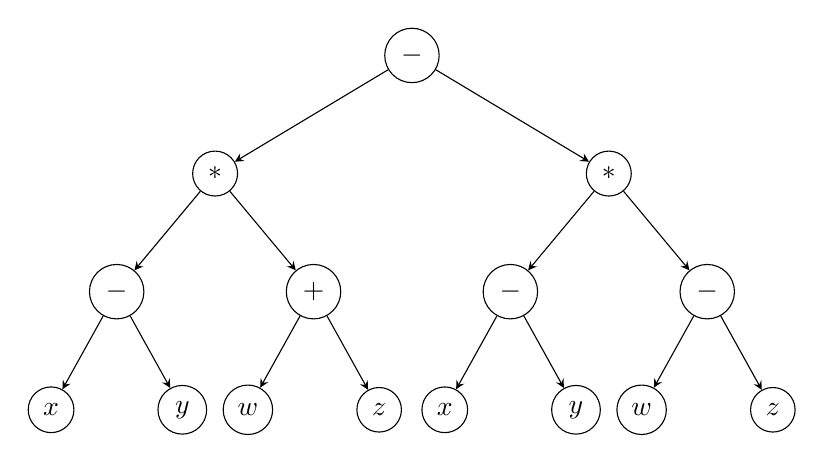
\begin{tikzpicture}
    [->,>=stealth,
    level/.style={sibling distance = 5cm/#1,level distance = 1.5cm},
    a/.style={text centered,align=center,circle,draw}]
    \node[a]{$ - $}
    child{node[a] {$ * $}
        child{node[a]{$ - $}
            child{node[a]{$ x $}}
            child{node[a]{$ y $}}
        }
        child{node[a]{$ + $}
            child{node[a]{$ w $}}
            child{node[a]{$ z $}}
        }
    }
    child{node[a]{$ * $}
        child{node[a]{$ - $}
            child{node[a]{$ x $}}
            child{node[a]{$ y $}}
        }
        child{node[a]{$ - $}
            child{node[a]{$ w $}}
            child{node[a]{$ z $}}
        }
    };
\end{tikzpicture}\\
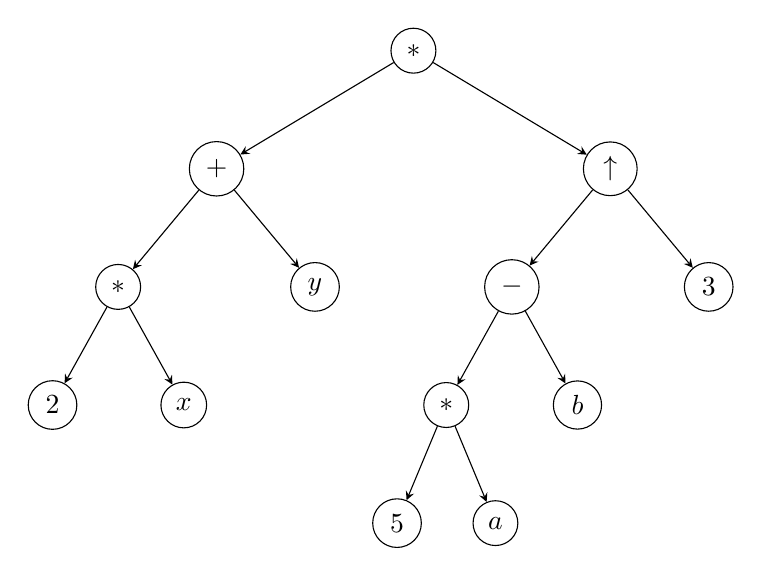
\begin{tikzpicture}
    [->,>=stealth,
    level/.style={sibling distance = 5cm/#1,level distance = 1.5cm},
    a/.style={text centered,align=center,circle,draw}]
    \node[a]{$ * $}
    child{node[a] {$ + $}
        child{node[a]{$ * $}
            child{node[a]{$ 2 $}}
            child{node[a]{$ x $}}
        }
        child{node[a]{$ y $}
            % child{node[a]{$ w $}}
            % child{node[a]{$ z $}}
        }
    }
    child{node[a]{$ \uparrow $}
        child{node[a]{$ - $}
            child{node[a]{$ * $}
                child{node[a]{$ 5 $}}
                child{node[a]{$ a $}}
            }
            child{node[a]{$ b $}}
        }
        child{node[a]{$ 3 $}
            % child{node[a]{$ w $}}
            % child{node[a]{$ z $}}
        }
    };
\end{tikzpicture}
\end{document}